\chapter{绪论}
\section{课题的研究背景与意义}
随着智能化设备的爆发,全球每天产生海量的数据,
这些数据来自大量的手机终端、传感器与其他的各种终端信息。
在海量信息的基础之上,深度学习模型蓬勃发展。
深度学习(Deep Learning)模型\cite{lim2020federated,DBLP:conf/www/LiuCBZL0C23}一般需要喂养大量规范化数据来保证模型可以学习
到有用的知识。
深度学习预训练模型已经应用到社会的方方面面,
包括人脸识别\cite{XDKD20241125005,XDDJ202424026,XAQY202411004}、
自动驾驶\cite{JSYJ20241211008,QCJS20241213002}、
生成式对话智能体\cite{10.5555/3295222.3295349,ZGGC202411001}、
医疗\cite{YXYZ202410001,ZXYX202409015,JSGG202405004}、
金融\cite{JLJX20241016005,DLXZ202407011}等等方向,
给人类社会的发展带来了巨大的便利。


模型的能力很大程度上取决于数据的质量,
然而这些数据的提供者大部分是来自于各种边缘设备,
现存的训练方法需要将客户产生数据集在中心聚集\cite{JSYJ201407002},然后在中心训练完整模型,
如图\ref{fig:1-1compare_2methods}所示,
客户端在中心化训练模型方式中仅仅需要将自己产生的数据收集,
然后上传给中心服务器即可。
诚然,基于中心化的训练方式可以大大提高模型训练效率,
但是也暴露了严重的隐私安全问题——所有的终端产生的数据都要在中心侧保存处理,
难免出现隐私泄露等等一系列问题\cite{RJXB202007012}。
中国在2021年制定了《中华人民共和国个人信息保护法》\cite{persionsafe}明确了个人信息的收集、存储、使用、
加工、传输、提供、公开等各环节的合规要求。
法律还规定了个人信息处理者的义务,以及对违法行为的处罚措施,旨在保护公民的隐私权。
《欧盟通用数据保护条例》\cite{eupersonsafe}(GDPR),该条例对个人数据的收集、存储、处理和传输
提出了严格的要求,
违规者将面临高额罚款。GDPR对全球范围内的信息安全管理产生了深远影响。
为了解决上述的隐私安全问题,谷歌在2017年提出了一种全新的深度模型训练的范式——
联邦学习\cite{mcmahan2017communication, karimireddy2020scaffold}(Federated Learning, FL)。
联邦学习是一种协同多个边缘设备训练模型,最终在中心服务器上聚合模型更新参数的
一种保护隐私的训练范式。
如图\ref{fig:1-1compare_2methods}所示,
在联邦学习的框架中,
客户端本地的数据不需要上传到服务器端,
随之而来的便是,模型的训练也同样需要在本地训练,
最终模型参数在中心侧聚合。
其核心之处在于,在不直接将边缘设备数据上传的情况下,实现了在中心侧模型的训练。
这也使得联邦学习广泛的应用在
医疗\cite{SJSJ202409003,JSJA20240510007,pfitzner2021federated,rieke2020future,sheller2020federated}、
金融\cite{DNXJ202403013,byrd2020differentially,imteaj2022leveraging,nevrataki2023survey}等高度注重隐私保护且又需要深度学习模型
赋能的场景。

虽然联邦学习可以跳过数据聚集过程而直接在端侧训练模型,然后更新参数到中心侧,
但是在实际过程中存在诸多挑战。
其中重要的一个是不同边缘设备产生的数据异构性问题。
在传统的中心化训练模型的过程中,我们将数据中的每个训练批次随机划分,
保证我们每次训练数据分布相似,也就是数据同构。
但是在联邦学习的范式中,数据孤立分布在边缘设备,很容易形成非独立同分布的数据集\cite{WXAQ202105007}
(Non-Independent and Identically Distributed, Non-IID)。
这将导致边缘设备训练的模型具有自己数据分布的参数特征\cite{li2020federated,li2022federated,huang2023stochastic},在聚合过程中导致
中心侧的模型泛化能力不行。例如在金融场景中,由于地理位置分布迥异,在西部地区
训练出来的模型与在东部沿海地区的模型必然存在显著的差异,
导致在聚合过程中影响整体模型的泛化能力,既不能很好的处理西部金融数据,也不能
处理东部数据的两难问题。
%ppppppppppppppppppppppppppppppppppppppp
\begin{figure}[htbp]
    \centering
    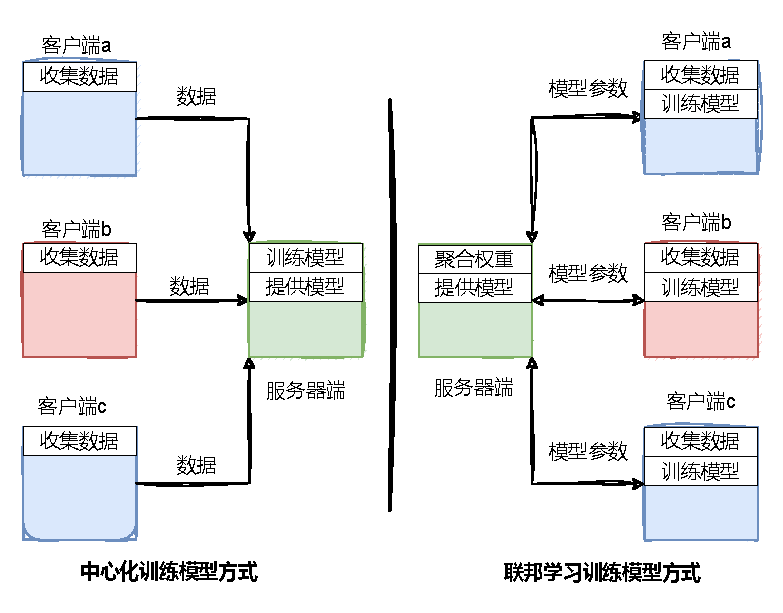
\includegraphics[width=0.9\linewidth]{chapter1/compare_fl_center.pdf}
    \caption{\label{fig:1-1compare_2methods}中心训练与联邦学习对比}
\end{figure}
%ppppppppppppppppppppppppppppppppppppppp

随着生成式模型的广泛应用,如今深度学习模型的参数规模越来越大,
另一个问题也随之而来。
边缘设备受限于资源限制已经无法承受训练现今越来越庞大模型\cite{cai2020tinytl, lee2019intermittent, DBLP:journals/imwut/LiuCZLWL0C21,DBLP:conf/infocom/WangXFLZ23,gobieski2019intelligence},
然而边缘设备的数据资源对于整个模型的训练有这重要的贡献。
这些问题主要集中在:
\begin{itemize}
    \item 计算资源受限\cite{cai2020tinytl,gobieski2019intelligence,lee2019intermittent}。现在的模型参数在千万百万级别都有,在一些比如手机、
    性能老旧的电脑、汽车传感器等等边缘设备上匮乏的资源计算空间与计算能力
    均不能支撑庞大的训练目标。
    \item 通讯成本限制\cite{WXAQ20241116001,JSJA2024061200B}。在联邦学习中边缘设备需要频繁与中心设备共享参数等
    信息,庞大的模型参数以为着在每个训练轮次都需要进行大量的高带宽的通讯,
    对于整个训练来说是庞大的开销。
    \item 隐私保护带来的数据异质性。由于数据不能在中心侧聚合导致每个终端
    都有自己特质的数据带来的训练偏差问题。
\end{itemize}

上述的问题本质都是异质性的问题,分别是设备资源异质性与数据资源异质性,并且二者往往
是同时出现的。
也是限制现阶段联邦学习发展的主要的瓶颈问题。
解决资源异质性问题为联邦学习在不同计算能力的终端侧应用铺平道路,使得联邦学习
的训练框架可以应用到各式各样的设备上,
不在因为计算资源不足的原因导致很多终端
设备的数据不能参与训练。
另一方面,解决数据异质性的问题使得联邦学习得到的模型的结果不在偏向于某些特定
数据,而是具有更好的泛化性,训练出的模型更能集合所有数据的特征。



\section{国内外研究现状}
时至今日,人工智能迅猛发展,保护隐私的分布式训练范式联邦学习成为了人们研究的
热点,
其中的热点问题数据异构和资源受限更是最新急需解决的重要问题。
Transformer架构\cite{vaswani2017attention}的出现更是将模型的规模提升到更高的级别,
并且训练数据的规模也得到了前所未有的增长。
这些架构在计算机视觉\cite{bai2023qwen},自然语言处理\cite{yang2024qwen2}取得了重大的成功,
模型规模的扩大,训练数据的增多对于联邦学习来说是一个巨大的挑战。
本章首先介绍传统的联邦学习,然后介绍资源受限联邦学习的处理方法,同时介绍数据异构的
解决方案。


\subsection{经典联邦学习方法}
\begin{table}[htbp]
    \caption{\label{tab:users_info_fl}不同用户的兴趣设备信息}
    \begin{tabularx}{\linewidth}{c|X<{\centering}|X<{\centering}|X<{\centering}}
        \hline
        用户 & 用户A & 用户B & 用户C \\ \hline
        设备 & 智能手机 & 个人电脑 & 智能汽车 \\ \hline
        运行内存 & 8GB & 32GB & 8GB \\ \hline
        计算能力 & 低 & 中 & 低 \\ \hline
        \multirow{2}{*}{兴趣} & 猫,松鼠, & 黑神话悟空, & 奔驰,理想, \\ 
        & 狗等小动物 & 穿越火线等游戏 & 特斯拉等汽车 \\ \hline
    \end{tabularx}
\end{table}

传统联邦学习是一种分布式机器学习技术,
其核心思想是在多个拥有本地数据的数据源之间进行分布式模型训练,
而无需交换本地数据。
各方仅通过交换模型参数或中间结果来构建基于虚拟融合数据下的全局模型,
从而实现数据隐私保护和数据共享计算的平衡。
传统的联邦学习的数据分布基于一个假设就是所有参与者提供的数据拥有相似
的数据分布结构,也就意味着所有边缘设备训练的数据是相近的。
另外一个默认的事实是,传统的联邦学习中每个边缘设备中训练的模型都是
一模一样的。
我们使用表\ref{tab:users_info_fl}不同用户设备和兴趣信息来说明传统联邦学习
在实际中遇到的困难,
与资源受限下联邦学习有明显的区别:
\begin{itemize}
    \item 边缘设备数据分布差异大。
    如表\ref{tab:users_info_fl}所示三个用户感兴趣的部分非常具有自己的特色,
    用户A对小动物感兴趣,A的数据分布对于动物数据占据大部分,使用A的数据训练的
    模型则偏向动物数据特征;
    同理,根据B、C的数据训练的模型也偏向各自的数据分布。
    例如,用户B的数据偏向游戏,而用户C则是偏向汽车领域。
    最终的模型则受到数据特征的影响泛化性下降。
    \item 边缘设备计算资源差距大。
    在表\ref{tab:users_info_fl}中所示三个用户使用的设备可以看出用户A使用的是
    智能手机\cite{kamal2018three}在运行内存还有是否存在可计算GPU上均不如用户B的个人电脑。
    也就意味着用户B可以训练比用户A更大的模型。
    反之,如果模型参数过大,用户A没有计算资源去训练中心侧需要的模型。

\end{itemize}

\subsection{基于知识蒸馏的资源受限联邦学习}
知识蒸馏是一种有效的方法来解决边缘设备的异构性\cite{gou2021knowledge}。
具体而言,FedDF\cite{DBLP:conf/nips/LinKSJ20}利用知识蒸馏
从一组使用客户端私有数据训练的本地模型中提取知识。
每个本地模型在未标记的公共数据集上的逻辑输出随后被用于通过知识蒸馏在服务器上
训练学生模型。
类似地,DS-FL\cite{itahara2021distillation}在服务器上采用未标记的公共数据集,
并引入了一种基于蒸馏的半监督联邦学习。
该技术旨在通过为公共数据生成伪标签来提高性能。
FedGKT\cite{he2020group}引入了组知识转移,即使在客户端没有任何公共数据的情况下,
也能有效地将知识从小型客户端模型转移到服务器上的大型模型。
Fed-ET\cite{cho2022heterogeneous}提出了一种加权共识蒸馏方案,
并结合了多样性正则化。
该方案通过利用小型客户端模型的知识来训练大型服务器模型。

知识蒸馏的方法能解决计算资源异构的问题,
但是由于在边缘设备需要选择合适大小的异构模型,
然而当前存在的模型不一定能最佳适配边缘设备计算资源的情况,
可能导致计算资源的浪费;
另一方面,知识蒸馏的方法需要中心侧拥有一定量的边缘设备数据相似的数据,
这些数据可以是有标签和无标签的。


\subsection{基于子模型抽取的资源受限联邦学习}
\label{sec:sub-extract}
%ppppppppppppppppppppppppppppppppppppppp
\begin{figure}[htbp]
    \centering
    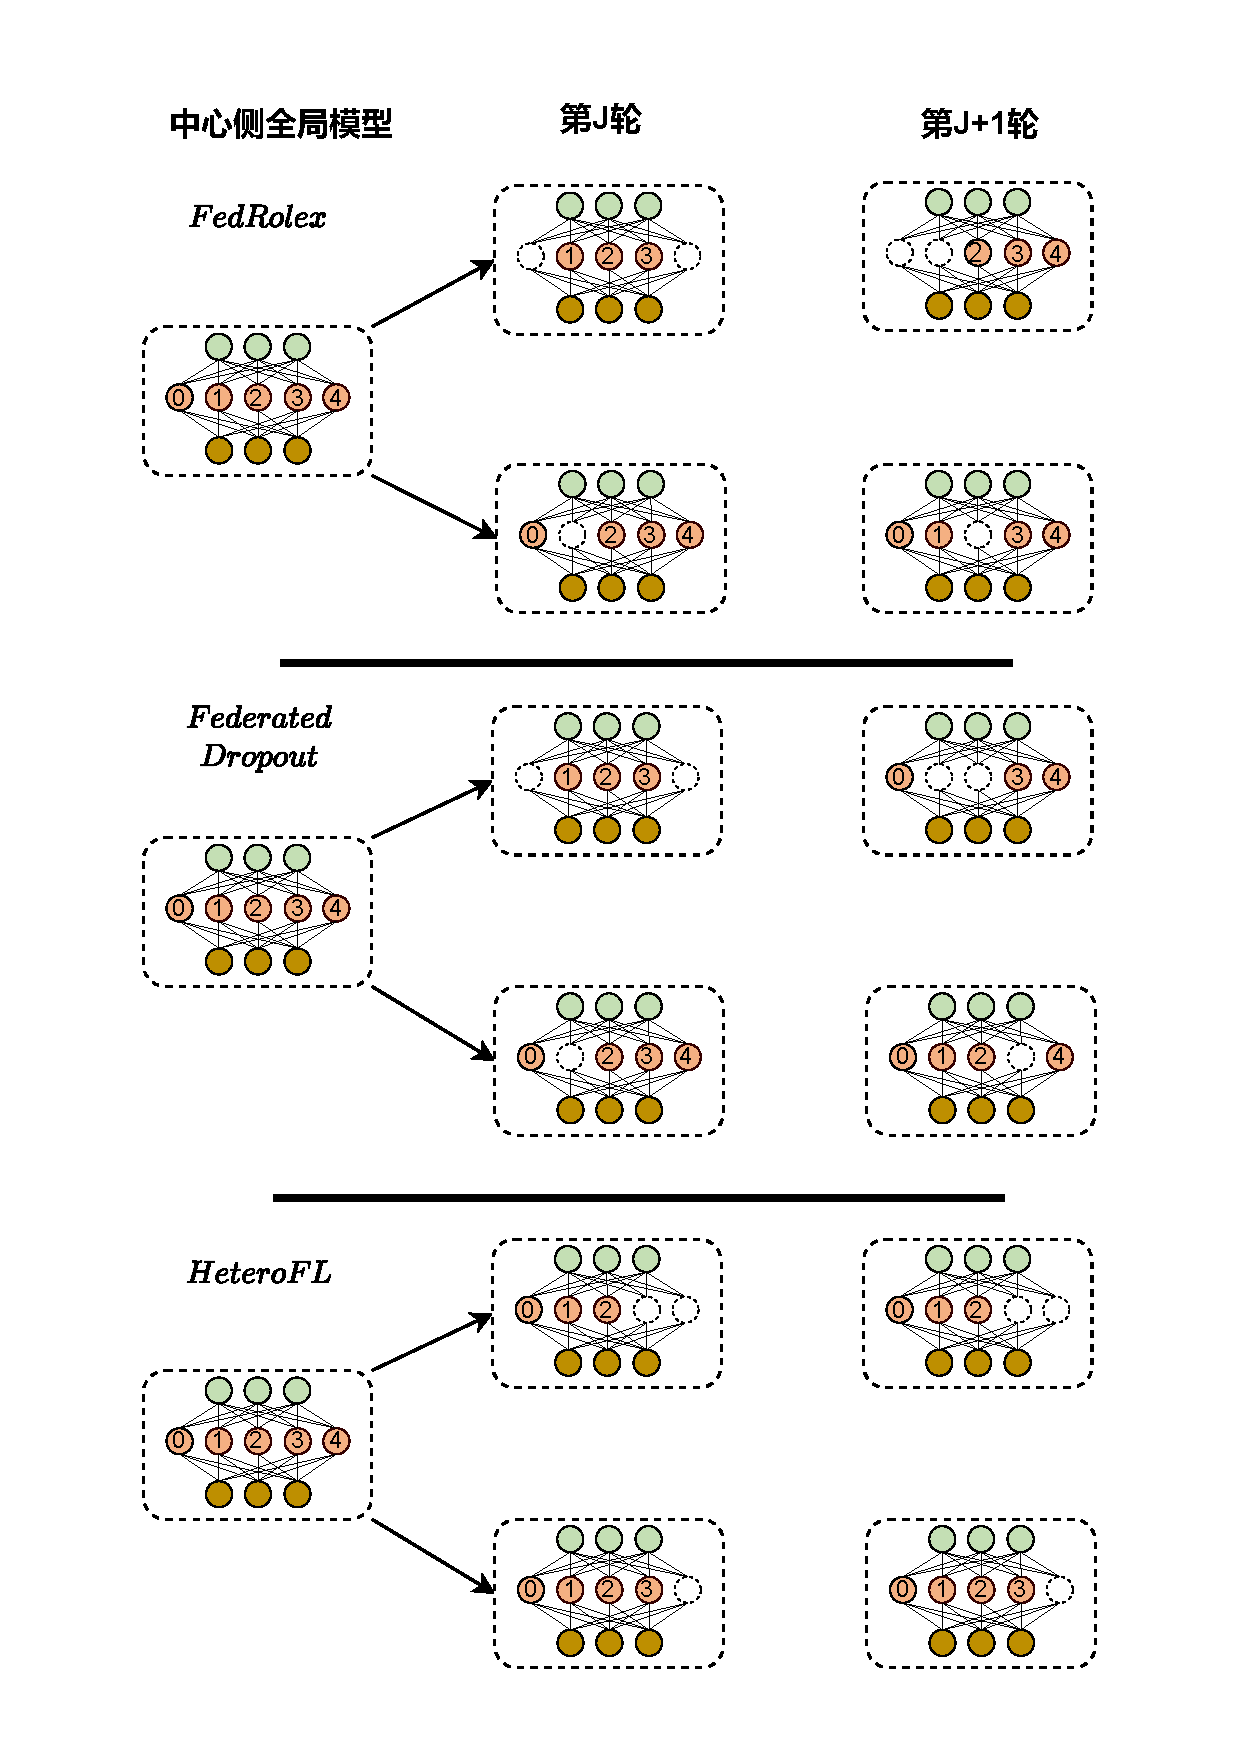
\includegraphics[width=\linewidth]{chapter1/threemotheds.pdf}
    \caption{\label{fig:1-1threemethods}子模型抽取的三种方法}
\end{figure}
%ppppppppppppppppppppppppppppppppppppppp

除了知识蒸馏方法之外,
对于边缘设备没有足够的计算资源来训练中心侧的全局模型的问题,
最简单的方法便是对于每个边缘设备按照其计算能力的大小从全局模型中抽取
相应大小的子模型以供边缘设备计算。
2021年Diao等人提出了一种基于预先分配规则的子模型抽取方法
HeteroFL\cite{DBLP:conf/iclr/Diao0T21},
对于深度学习模型此方法依据边缘设备的计算能力按照全局模型每层神经元的先后顺序
抽取前面的神经元组成子模型层,
每层按照上述的思路进行抽取,
最后组成完整的子模型发送给边缘设备。
如图\ref{fig:1-1threemethods}中最下方所示,
每个轮次中同一个客户端所获得的子模型都是相同的构造,
不会因为通讯轮次不同而发生改变,
图中不管是第$J$轮或者是$J+1$轮都是$\{ 0, 1, 2 \}$(上面客户端)和
$\{0, 1, 2, 3 \}$(下面客户端)参与训练并且保持不变。
HeteroFL横向的抽取每层的神经元巧妙的解决了边缘设备无法计算全局模型的困境,
并且可以根据边缘设备自己的计算能力设定需要抽取子模型的大小,具有一定的自适应性。
同期的方法FjORD\cite{DBLP:conf/nips/HorvathLALVL21}使用了和HeteroFL
相同的思想来解决资源受限的联邦学习场景。
这种方法有个很明显的缺点,处于后面的神经元在整个联邦学习的训练过程中被训练的
次数远少于位于每层前面的神经元。
在图\ref{fig:1-1threemethods}所示中,
最后一个神经元永远没有得到训练的机会。

为了解决上述按照顺序挑选神经元的缺点,
一种简单的按照深度学习模型每层随机挑选神经元的方法被提出了。
简单来说就是在每层的基础上使用随机的方法根据边缘设备的能力来挑选神经元,
我们称这种方法为Federated Dropout\cite{caldas2018expanding}。
这种方法大致解决了每个神经元训练次数不一致的问题,
但是这种随机的方法不能保证每个神经元训练的次数一定是相同的,
只是在概率上保证大概率是一样的。
如图\ref{fig:1-1threemethods}中所示,
在不同轮次的抽取过程中,
相同两个轮次之间的子模型抽取没有任何的规律可言,
都是通过随机数产生的。
也就是Federated Dropout方法存在很大的不稳定性,
模型训练的结果存在一定的随机性。

Alam等人提出了一种解决基于顺序方法训练不均的方法叫做
FedRolex\cite{DBLP:conf/nips/AlamLYZ22},
此方法解决了HeteroFL与FjORD方法中的问题。
FedRolex不在是每个边缘设备都是固定的按照顺序的分配子模型,
而是在HeteroFL的基础上,按照当前训练的轮次,
在上一个轮次的基础上将每层挑选的神经元的序号向后平移一个单位,
这样在每个轮次训练过程中,训练的神经元都是上一个轮次训练的
下一个序号的神经元,当序号达到末尾的时候就挑选头部的神经元。
保证了每个神经元都可以均匀的参与到模型的训练过程中。
如图\ref{fig:1-1threemethods}中所示,
上一轮的神经元序号在本层平移到一下个序号上,
在图中就是从序号$\{1,2, 3 \}$变成了挑选序号为
$\{2, 3, 4 \}$的神经元,
保证了每个神经元都可以得到平均的训练。

上述所提及到的方法属于在深度学习模型的横向进行了子模型抽取,
而Kim等人在2023年提出了基于深度抽取子模型的方法\cite{kim2023depthfl}。
此方法不同于上述的方法在横向在每层的维度上抽取特定的神经元,
而是根据边缘设备的计算能力在深度上抽取不同的层来组成子模型。
按照深度方向抽取有一些缺点,不能灵活的按照边缘设备的计算能力
抽取子模型,
因为深度学习模型多个层组层一个逻辑上的块,所以应该在块的维度上抽取,
这样会导致子模型的抽取不自由。



\section{本文研究内容}
本文主要研究边缘设备计算能力受限情况下联邦学习框架研究,
主要是基于子模型抽取这一类方法的延续,并在子模型抽取的过程中考虑到
边缘设备数据异构分布做出优化。
% 在专门解决资源受限和数据异构结合了知识蒸馏方向的研究。
我们可以看到在以上的子模型抽取的方法中,都是根据预先制定好的规则去
实现每个轮次如何挑选子模型,
也就是意味着在实验前我们可以预测每个轮次所抽取的子模型,
这种设计没有根据边缘设备数据的异质性,
本文主要将预先设定的抽取规则转变为自适应的抽取规则,
具体的研究内容如下:
\begin{itemize}
    \item 本文在子模型抽取的所有方法中,首先提出了动态的在每轮
    通讯中自适应的去抽取最合适子模型的方法,改进了预先制定规则
    方法,提高了资源受限联邦学习场景下训练的模型上限。

    \item 本文提出了一种基于边缘设备数据分布来动态抽取子模型的方案FedDSE。
    具体来讲FedDSE摆脱了提前定制的抽取方案,
    而是根据边缘设备在自己终端处数据推理运算得出的神经元激活值
    作为挑选子模型的标准。
    神经元在不同数据集上的表现出不同的激活值,
    激活值表示了对于当前数据的敏感程度,
    筛选出激活值大的神经元作为子模型的组成部分,
    可以避免神经元在训练过程中的冲突情况,
    从而取得较好的效果。
    并且充分考虑了联邦学习在实际情况中的数据异质性问题。

    \item 从子模型与中心侧模型优化方向作为出发点,
    本文又提出了一种基于梯度的联邦学习框架。
    在FedDSE中我们考虑了边缘设备数据异构的情况,
    基于此提出了激活值作为参考挑选神经元的思路,
    在此基础上提出了基于反向传播中梯度挑选神经元的方法FedGSE,
    以梯度为考虑要点可以是参数优化方向与中心侧模型一致。
    % 但是还是不可避免的没有解决数据异构带来的对模型最终泛化能力影响的问题,
    % 对此提出了一种基于梯度和知识蒸馏的解决资源受限和数据异构问题的联邦学习方法
    % FedKDGSE。
    此方法首先在中心侧构建了一个全局数据集,这个数据集放在中心侧,
    然后筛选出合适部分的子数据集在全局模型上反向传播得到梯度,
    计算出的梯度作为挑选标准筛选子模型,
    由于反向传播过程需要庞大的计算能力,
    所以将这一过程在中心侧实现,全局数据集正好可以作为反向传播使用的数据。
    % 由于全局数据集的存在,我们在中心侧对聚合的模型做知识蒸馏,
    % 这个过程可以改变数据异构带来的偏差。
    
\end{itemize}

\section{本文结构安排}
本文共包括五个章节,每个章节的主要内容如下:

第一章:绪论。
绪论主要介绍了联邦学习出现的背景以及要解决的问题,
联邦学习发展至今遇到的关键技术难题;
然后介绍了国内外解决技术难题的论文与相关工作与不足之处;
最后引申出本文主要做出的贡献以及成果。

第二章:理论技术与公式化表达。 
本章主要介绍本文中用到的相关技术的理论化表达以及相关的优化目标,
为本文的表达提供前置知识。
首先介绍联邦学习经典的联邦学习以及共同的优化目标函数,
然后介绍本文中需要训练的深度学习模型卷积神经网络以及神经元的定义。
% 最后介绍蒸馏学习的发展与优化目标。

第三章: FedDSE方法详细阐述。
本章将介绍本文提出的方法FedDSE。
首先会介绍在以往的方法中的问题做出分析,
% 然后预实验证明此方法的效果,
通过思想实验与简单的预先实验来揭示此前方法中存在的问题,
然后提出FedDSE方法详细实现方式完整的讲述基于激活值的子模型抽取方法,
在详尽的实验中证明方法的可靠性与优越性,
通过大量的消融实验证明参数的重要程度,
最后总结本章方法的优缺点。

第四章:FedGSE方法详细阐述。
本章内容在第三章的基础上做出改进解决了资源受限的问题,
% 而且对于数据异构分布也做出了应对的方案。
从一个新的视角优化策略方向考虑解决问题的方式,
之后详尽的介绍了FedGSE方法公共数据集的收集,
相似数据生成,子模型筛选等具体细节,
然后从理论上分析了此方法的可行之处,
最后通过相关的实验证明了此方法。
并通过消融实验对比了众多参数的重要性程度。
最后总结方法的优缺点。

第五章:总结与展望。
本章概括性的总结了本文方法的技术要点与创新性的地方,
并且提出了方法的不足之处与未来需要改进的地方。
为该领域的发展提供了后续研究发展的启发。